\section{Hyperparameter Optimization}

There are five hyperparameters which influence the execution of \textit{SPIND}. The size of the initially created chunks, the maximal number of values which are kept in main memory during the sorting phase per thread, the maximal number of files which are merged at once, the total queue size over all relations during candidate validation and the degree of parallelization in all execution phases. Leveraging Bayesian optimization \cite{shahriari2015taking}, we seek to efficiently and iteratively identify parameter configurations that minimize the execution time of \textit{SPIND} of various datasets. We lower bound the chunk size by 10,000 to avoid creating a massive amount of files the upper bound is set to 100 million. The maps used during sorting are limited between 100,000 and 50 million to find a balance between a large number of files being written and a safe number under the main memory threshold (20 GB). The number of simultaneously merged files is lower bounded by two and upper bounded by 2,000 to not put too much pressure on the file system. Relation buffers during the validation are upper bounded by 1 million. Finally, the degree of parallelization is upper bounded by the number of virtual threads of the executing machine.

The experiments are conducted using the datasets \textbf{EU}, \textbf{US}, and \textbf{TPC-H 1}. These datasets contain different structures and using all of them will help us finding robust settings that do not over fit some precise dataset structure. In total 732 samples where calculated after which we reached a 95\% certainty, that the maximum has been found.

A first observation is that the parallelization degree has a clear negative correlation with the execution time. We find that the fastest executions use at least 9 threads, regardless of how the other four parameters are set. Once we find suitable settings for the other hyperparameters, we will investigate the precises effectiveness of parallelization.

A next observation yielded that the chunk size is the second most important variable. While smaller chunks strictly correlate with the total number of files being created and therefore also the I/O overhead, we find an optimum at a chunk size of five to seven million which is also robust for \textbf{Musicbrainz}, \textbf{TPC-H 10} and \textbf{UniProt}. A smaller chunk size enables more tasks to be processed in parallel which has been shown to overcome the I/O operations at some point.

\begin{figure}[t]
    \centering
        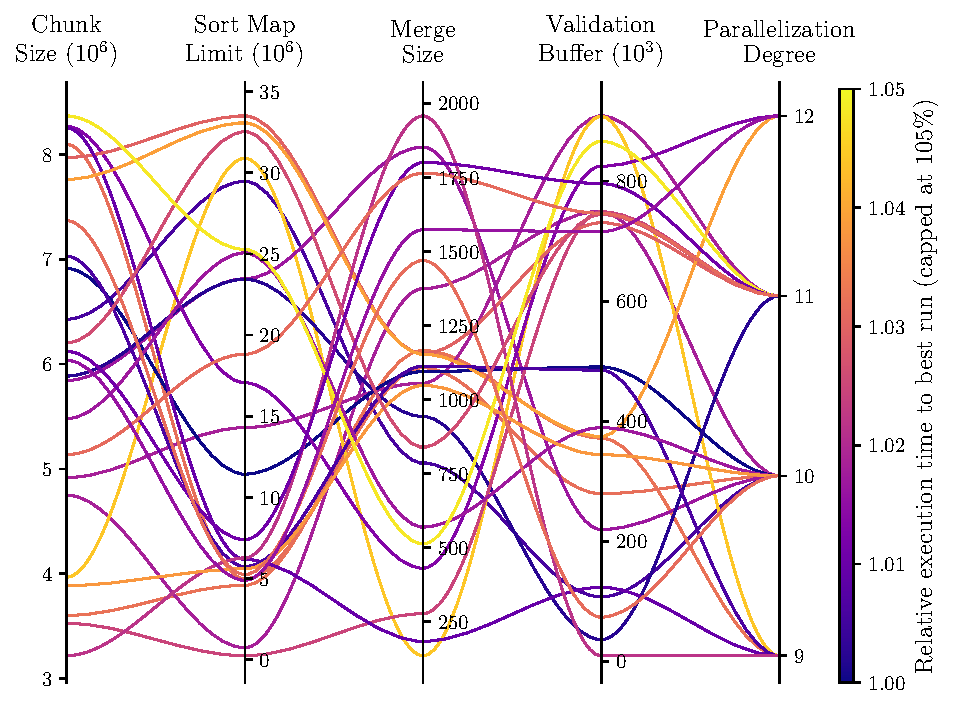
\includegraphics[width=.48\textwidth]{figures/Hyperparameters.pdf}
    \caption{Sub-sampled visualization of hyperparameter influence on the execution time of \textit{SPIND}. Optimization conducted on the datasets \textbf{EU}, \textbf{US} and \textbf{TPCH}.}
    \label{fig:hyperparameters}
\end{figure}

In Figure \ref{fig:hyperparameters} we find a parallel coordinates plot of the sub-sampled hyperparameters. We have excluded all executions using less than 9 threads as well as executions with very large or very small chunk sizes. As a last step we only view the runs, which are in close proximity (5\%) to the best performing execution. Each line represents a single execution and is colored based on the relative time to the best execution. After the performed sub-samples we can not find clear structures, which can be explained by the different datasets and that some configurations work well for one of them while performing poorly on others. We have tried to find a stable setting as a standard for the parameters and decided to use a chunk size of 6 mil, sort maps are limited by a total of 25 mil, the number of simultaniously merged files is capped at 1,200, the validation buffers are limited to 250,000 and the parallelization is set to 12, its maximum.



In Figure \ref{fig:chunk_size} we can observe the relative change in the number of files created under changing chunk sizes (left) and the relative execution times compared to the longest run (right). For these experiments, we always average the execution of three runs.

